\BiChapter{控制论与机器学习}{CSandML}
控制论其本质,在于利用已有的信息抑制系统熵的增加\citeup{weina},需要注意的是,这里的熵并不是指热力学中的热力熵或信息论中的信息熵,而应理解为熵的原始定义,即对混乱的度量。既然是度量,便需要一个准则,正如测量一个物体的长度需要一把刻度尺,但不同的刻度尺将得到不同的测量结果,同理,对混乱的不同定义,也将得到不同的控制效果。例如,在温度控制系统中,让温度保持在一个较高的温度或较低的温度均是抑制熵增的行为,因为两者对熵的定义不同。对于孤立系统,熵总是朝着增加的方向移动,但也有例外,此时系统必须是非孤立的,能够收到外界的控制,比如有机体具有熵减趋势,因为DNA是有序的(尽管我们目前仍无法完全理解它),其中起到控制作用的外力是自然选择。控制论所要做的,便是引入外力作用,即反馈,或者说控制环节,以之降低系统的混乱程度,得到我们的期望输出。

\BiSection{白盒模型与经典控制论}
x经典控制论中,为了实现对一个系统的控制,我们往往需要先由系统的结构开始分析,利用牛顿力学、电磁原理、热力学等物理原理对系统特性建立微分方程,将其转换为复域的传递函数后,再利用根轨迹或频域分析设计控制环节。如图\ref{img:RLC} 所示的简单RLC网络中,假定我们以$u_i(t)$作为输入,$u_o(t)$作为输出,那么此时我们所拥有的信息是整个系统的结构,所需要抑制的混乱就是控制$u_0(t)$朝着我们的期望输出迈进。

\begin{figure}[htbp]\label{img:RLC}
\centering
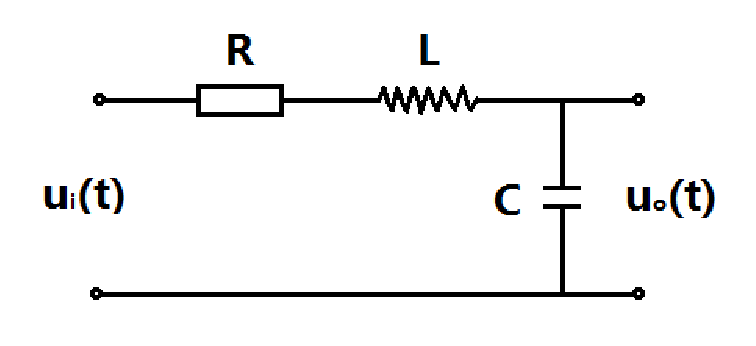
\includegraphics[width=0.5\textwidth]{CSandML/RLC.eps}
\caption{简单的RCL网络}
\end{figure}

由于这个系统的结构是已知的,整个系统对于我们而言相当一个白盒。为此,我们可以很容易地根据基尔霍夫回路电压定律建立方程
\begin{equation}\label{equ:KVL}
u_L(t) + u_R(t) + u_o(t) = u_i(t)
\end{equation}
进一步利用电感特性、电容特性、欧姆定律,式\eqref{equ:KVL}可以进一步推导为
\begin{equation}
LC\frac{d^2u_o(t)}{dt^2} + RC\frac{du_o(t)}{dt}  + u_o(t) = u_i(t)
\end{equation}
此时,输入输出的微分方程已建立,下一步便是经典控制论的内容,我们并不打算继续展开细说。在这个例子中,我们可以看出,白盒模型对整个系统是了如指掌的,是可以对其建模的。此时,“利用已有信息抑制系统的熵增”相当于,对系统建立传递函数(利用已有信息),设计控制环节使我们能得到期望输出(抑制熵增)。

\BiSection{灰盒模型与系统辨识}
x牛顿一生的工作对自然科学的贡献是无以衡量的,但牛顿生活的时代忽视了一些重要的东西---统计的概念。在牛顿力学中,有一个前提,系统的状态是可测量的,因此,牛顿力学基于一个已给定的精确初始状态之上对系统分析。然而,物理的测量从来都不是精确的,我们对世界的观察也总是片面而不确定的,世界对我们而言是未知的,我们无法完全确定事物的运作机理。例如图\ref{img:RLC} 中的电阻R,R=50$\Omega$ 并不是一个严谨的说法,我们不知道物体细分到最小粒子(如果存在的话)后事物是否变得精确,但就目前人类所拥有的知识而言,阻值为50$\Omega$的电阻是不存在的。我们平常所说的50$\Omega$电阻只是一个统计概念,即电阻在50$\Omega$左右的统计结果。延伸到整个系统,图\ref{img:RLC} 的网络也变得不确定,R、L、C均是不精确的值,此时系统变为一个灰盒模型。所谓灰盒模型,即系统的一部分内容是未知的,另一部分内容是已知的的,例如这里,尽管R、L、C的精确值是未知的,但我们依然可以知道其数值的大致范围。

倘若我们再推广一步,R、L、C的大致范围我们也不知道,如何设计该系统的控制环节便是系统辨识所要研究的内容。系统辨识领域中的一个重要的话题是如何解析出一个含有未知参数的系统结构,如果我们可以获取系统的输入输出样本,利用这些样本,配合上含有未知参数的系统结构方程,采取恰当的拟合方法,如最小二乘以及极大似然等,最后可以获取未知参数的近似解,使得这个灰盒模型的灰色褪去(但不会褪为白盒模型),进一步便可设计系统的控制环节。
\BiSection{黑盒模型与统计机器学习}
x白盒模型与灰盒模型的讨论均是基于一个前提:我们知道系统整体模型框架,只是某些参数有可能是未知的。但这个前提在实际生活中往往是不成立的,很多时候,我们非但不知道系统的参数,甚至连系统的模型也知之甚少,此时的系统相当于一个黑盒,我们无法了解其内部结构。例如,判断一封100字的邮件是否为垃圾邮件,假设这个行为可以用一个函数来描述,即这个决策背后存在一个真理(或者说函数),通过它,我们输入100个字符,函数的输出告诉我们这封邮件是否为垃圾邮件 ,那么我们便可以通过这个函数来描述这个系统。可以肯定的值,这个函数在邮件完全可分(即不存在一些可能是或可能不是垃圾邮件的情况)的前提下是存在的,因为字符编码是有限的,只需穷举即可得到这个函数的决策面。但这个方法并不现实,假使所有的汉字只有2000个,那么100字的中文邮件将有$2000^{100}$种可能,要穷举是不可能的。另一种做法是寻求语法结构,先对这100字进行分词,再进行语义分析,这个过程也可以描述为一个函数映射过程:假设函数$f(x)$代表分词,$g(x)$代表语义分析,$y$代表系统输出,那么系统的模型可以表述为$y = g[f(x)]$。这种想法早在二十年前就被抛弃,因为自然语言含有强烈的上下文气息。例如在“冬天能穿多少穿多少,夏天能穿多少穿多少”这个例子中,同一句“能穿多少穿多少”在不同的上下文中含有不同的意义。尽管我个人认为这种上下文背后也必然存在一个因果关系,但这种因果关系是在是太难寻找了,所以这种方法也不是一个可行的方案。

统计机器学习的做法是,假定一个模型(这个模型与系统本质的模型关联并不大),利用大量样本训练假设的模型,最后将训练完毕的模型作为本质模型的逼近。与之前讨论的系统辨识相比,两者在训练阶段是类似的,均是利用样本进行参数整定,不同点在于,系统辨识是训练带有强烈先验的模型(比如由具体物理原理推导出的传递函数)的参数,而统计学习训练的是假设模型(比如高斯模型、隐式马尔可夫模型、神经网络、支持向量机等)的参数。

回到垃圾邮件分类的例子中,统计机器学习的一种解决方案是利用朴素贝叶斯分类,这种方法中,所假设的模型是朴素贝叶斯模型。我们首先建立一个含有$d$个元素的垃圾邮件特征字典,比如$\{$ 购买、大促销、店庆$\cdots \}$,此时,任何一封邮件都可以用一个$d$维列向量表示。例如,某封邮件在字典中的元素只包含“购买”,而其他的元素均不包含,那么这封邮件便可以表示为
\begin{equation}
x = [1, 0, 0, \cdots , 0]^T
\end{equation}

如果我们有大量垃圾邮件样本,我们不难统计出字典中各个元素在垃圾邮件中的出现概率$p(x_i|y=1)$,其中,$y$代表样本的标签,若该样本是垃圾邮件,则$y=1$,反之$y=0$,$x_i$代表字典中的第$i$个元素,例如,我们的字典中,$x_1$ = “购买”。建立样本的描述方式后,我们采用朴素贝叶斯公式,计算样本为垃圾邮件时的概率分布
\begin{equation}\label{naiveBayess}
\begin{split}
p(x|y=1)&= p(x_1, x_2, \cdot, x_d|y=1)\\
&=p(x_1|y=1)p(x_2|y=1)\cdots p(x_d|y=1)
\end{split}
\end{equation}
显然,式\eqref{naiveBayess}在数学上只有在$x_i$均独立时才成立,而本质上,$x_i$并不是独立的(因为存在上下文),这里本应使用全概率公式,而我们之所以假设$x_i$独立的原因是这样做可以降低模型的复杂度。所以说,在统计学习中,假设模型与本质模型的关联往往不大。

模型训练完毕后(即计算$p(x_i|y=1)$),对于一封新收到的邮件,我们只需使用贝叶斯公式即可计算该邮件是垃圾邮件的概率
\begin{equation}
\begin{split}
p(y=1|x) &= \frac{p(x|y=1)p(y=1)}{p(x)}\\
&=\frac{\prod_{i=1}^d p(x_i|y=1)}{\prod_{i=1}^d p(x_i|y=1) + \prod_{i=1}^d p(x_i|y=0)}
\end{split}
\end{equation}
统计学习更像是一种假设检验,本例子中的朴素贝叶斯,完全抛弃了语义分析,这并不符合自然语言的原理。但实际中,尽管这个模型并不是本质模型,但逼近效果足以让人接受,能工作得很好,因此被很多邮件厂商所采用。

\begin{figure}[htbp]
\centering
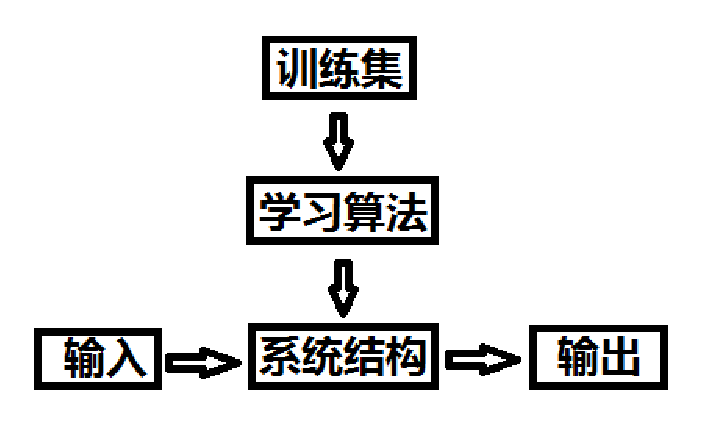
\includegraphics[width=0.4\textwidth]{CSandML/ML.eps}
\caption{机器学习系统框图}\label{img:ML}
\end{figure}

如果一定要对机器学习下一个定义,我认为Tom.Mitchell的描述比较恰当:对于某类任务T和性能度量P,如果一个计算机程序在T上以P衡量的性能随着经验E而自我完善,那么我们称这个计算机程序从经验E中学习\citeup{tomML}。如果将这段话转化成系统框图,则如图\ref{img:ML} 所示。

\BiSection{本章小结}
x精确性只存在于数学中,现实世界充满了不确定性,难以寻找事物背后的机理。统计学习绕过这套机理,根据设计者的意愿,假设一个模型,利用这个模型逼近事物的机理,相当于把世界看成一个黑盒,并不打算去探索黑盒的内部结构,而是仿造一个黑盒来模拟其工作原理。